\documentclass[11pt,letterpaper]{article}
\pagestyle{plain}
\usepackage{amsmath}
\usepackage{amssymb}
\usepackage[utf8]{inputenc}
\usepackage{times}
\usepackage{hyperref}
\usepackage{graphicx}
\usepackage{wrapfig}
\usepackage{listings}
\usepackage[usenames,dvipsnames]{xcolor}
\usepackage{setspace}
\usepackage{python_syntax}
\usepackage[sort&compress]{natbib}
\usepackage{bibentry}
\usepackage{todonotes}
\usepackage{url}
\usepackage[compact]{titlesec}
\titleformat{\subsection}[runin]
{\normalfont\large\bfseries}{\thesubsection}{1em}{}
\titleformat{\subsubsection}[runin]
{\normalfont\large\bfseries}{\thesubsubsection}{1em}{}
\usepackage{enumitem}
\usepackage[
top    = 1in,
bottom = 1in,
left   = 1in,
right  = 1in]{geometry}
\usepackage{caption}
\captionsetup{belowskip=0pt,aboveskip=0pt}
\linespread{0.92} % NSF allows up to 6 lines per inch.  
\def\UrlFont{\em} % Italicize all URLs.  
\frenchspacing
\setlist{nolistsep} % or \setlist{noitemsep} to leave space around whole list
\lstset{
	basicstyle=\small\ttfamily,
	breaklines=true,
	language=Python,
	}
\let\verbx\lstinline
\newcommand{\bfhead}[1]{\noindent \textbf{#1:}}

\begin{document}

\section{Abstract}
Rigorously validating a scientific model's explanatory power requires comparing its predictions against empirical data on an ongoing basis. 
However, model validation remains an informal and incomplete process, especially in fields like neuroscience where the available data is growing rapidly.   
This has made it difficult to develop a contemporary understanding of a model's strengths and weaknesses, to adequately compare competing models, to determine the state-of-the-art, and to precisely identify open modeling problems.

Software engineers validate software by developing simple executable tests, called ``unit tests'', that individually check a portion of a program against a single correctness criterion. Suites of such unit tests that collectively capture the desired program behavior provide evidence for its validity and correctness. Drawing inspiration from this practice, we develop the \textit{SciUnit} framework for developing suites of ``model validation tests'' -- 
executable functions, here written in Python, that compare model predictions against single empirical observations to  produce a score indicating agreement between the model and the data. Suites of such validation tests are used as a summary of modeling progress within a scientific community. 
Building on this framework, we develop \textit{NeuronUnit}, a library that supports validation testing for neurophysiology\todo{is this accurate?}.

% Section 1.
\section{Introduction}
Neuroscientists construct quantitative models to coherently explain observations of neurons, circuits, brain regions and behavior. 
These models can be characterized by their \textit{scope}: the set of observable quantities that the model can generate predictions about, and by their \textit{validity}: the extent to which these predictions agree with empirical observations of those quantities.

Today, scientists contribute a new model to the research community by submitting a paper describing how the model works, along with selected figures demonstrating its scope and validity and comparing its validity to other models with the same scope. Reviewers are then responsible for discovering relevant data and competing models that the paper did not adequately consider, drawing on their knowledge of prior publications. Unfortunately, in many areas, the number of publications being generated every year can overwhelm  even the most conscientious  scientists \todo{citation/stats?}. 

%This suggests that tools that help researchers answer questions like these could help readers and reviewers develop a more comprehensive understanding of the state-of-the-art and improve the quality of the research being published as a result: to renewed calls for tools that help researchers . 

Unfortunately, there are few alternatives to a comprehensive literature review available when scientists need to answer questions like these:
\begin{itemize}
\item Which models are capable of predicting the quantities I am interested in?
\item Which metrics should be used to evaluate the goodness-of-fit between these models and  data?
\item How well do these models perform, as judged to these metrics, given currently available data?
\item What other quantities can and can't these models predict?
\item What observations are not adequately explained by any available model?
\end{itemize}

%These questions are particularly relevant for young scientists and  scientists aiming to enter a new research area to answer.

%understanding of the state-of-the-art from publications containing only a few pieces of data, and then only that data available at the time of publication. 

%These demonstrations also quickly go out of date. Finally, there is no easy way to summarize and compare the claims being made in modeling papers in order to synthesize an understanding of a research area as a whole. 
%A strength of publications are their focused descriptions of new data and models. 
%A weakness, however, is that evaluating the scope and validity of models against known data is intractable using a body of publications alone.

Professional software developers face similar issues. They must understand the scope of each component of a software project and validate it by measuring how well each component achieves its stated goals. But software developers do not validate components by simply choosing a few interesting inputs and presenting the outputs to reviewers. Rather, they typically follow a \emph{test-driven development} methodology by creating a suite of executable \emph{unit tests} that collectively specify the scope of each component and validate the functionality of its implementation as it is being developed and modified. Each test individually checks that a small portion of the program meets a single correctness criterion. For example, a unit test might verify that one function within the program correctly handles malformed inputs. Collectively, the test results serve as a summary of the validity of the project as it progresses through its development cycle. Developers can determine which features are unimplemented or buggy by examining the set of failed tests, and progress can be measured in terms of how many tests the program passes over time. This methodology is widely adopted in practice \cite{tdd}\todo{cite tdd}.

%publications would be analagous to user manuals, rather than rigorous justifications that a program meets a specific specification. Unit tests serve this purpose for software, so we argue that the validation of neuroscience models by means of executable tests would be useful to scientists as a supplement the publication system.

Test-driven methodologies have started to see success in science as well. Modeling competitions in neuroscience, for example, are typically organized around a collection of simple validation criteria, implemented as executable tests. These competitions continue to drive important advances and improve scientists' understanding of the relative merits of different models. For example, 
the quantitative single neuron modeling competition (QSNMC)\cite{jolivet_quantitative_2008} investigates the complexity-accuracy tradeoff among reduced models of excitable membranes; 
the ``Hopfield'' challenge\cite{hopfield_what_2000} tested techniques for generating neuronal network form given its function; 
the Neural Prediction Challenge sought the best stimulus reconstructions, given neuronal activity\cite{neural_prediction_url}; the Diadem challenge is advancing the art of neurite reconstruction\cite{diadem_url}; and 
examples from other subfields of biology abound\cite{dream_url}.

% \begin{figure}%{r}{0.6\textwidth}
% %\vspace{-38px}
% 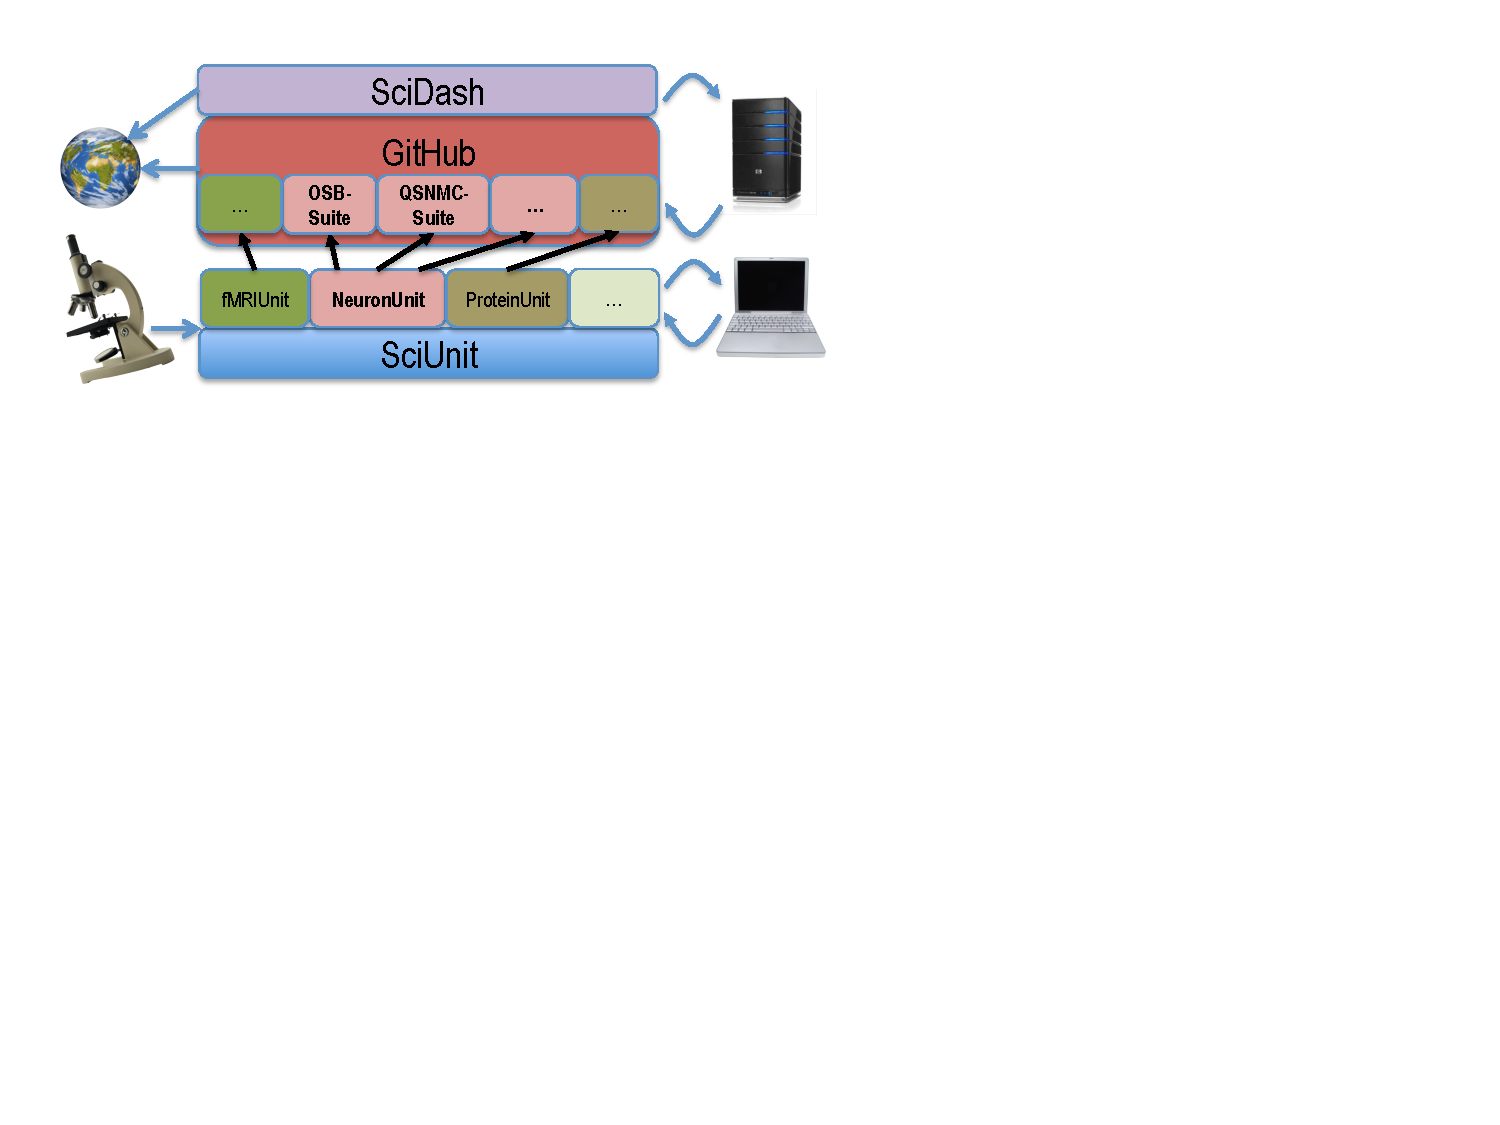
\includegraphics[scale=0.75]{sciunit_overview.pdf}
% \caption{Proposal overview. 
% \small{i) The \textit{SciUnit} framework can generate discipline-specific libraries for tests generation and model interfacing.  
% \textit{NeuronUnit} is proposed and described here.  Experimental data guides test development; model generation informs and is informed by these \textit{SciUnit} libraries.  
% Each \text{SciUnit} test suite repository on GitHub is indexed by the \textit{SciDash} web application.  
% Test suites for OSB and QSNMC (described in the text) are being built. 
% \textit{SciDash} automatically runs the test collections in each suite and publicly displays the results.}}
% %\vspace{-10px}
% \label{fig:sciunit_overview}
% \end{figure}
% \leavevmode
% \vspace{-0px}
\begin{figure}
\vspace{-38px}
\centering
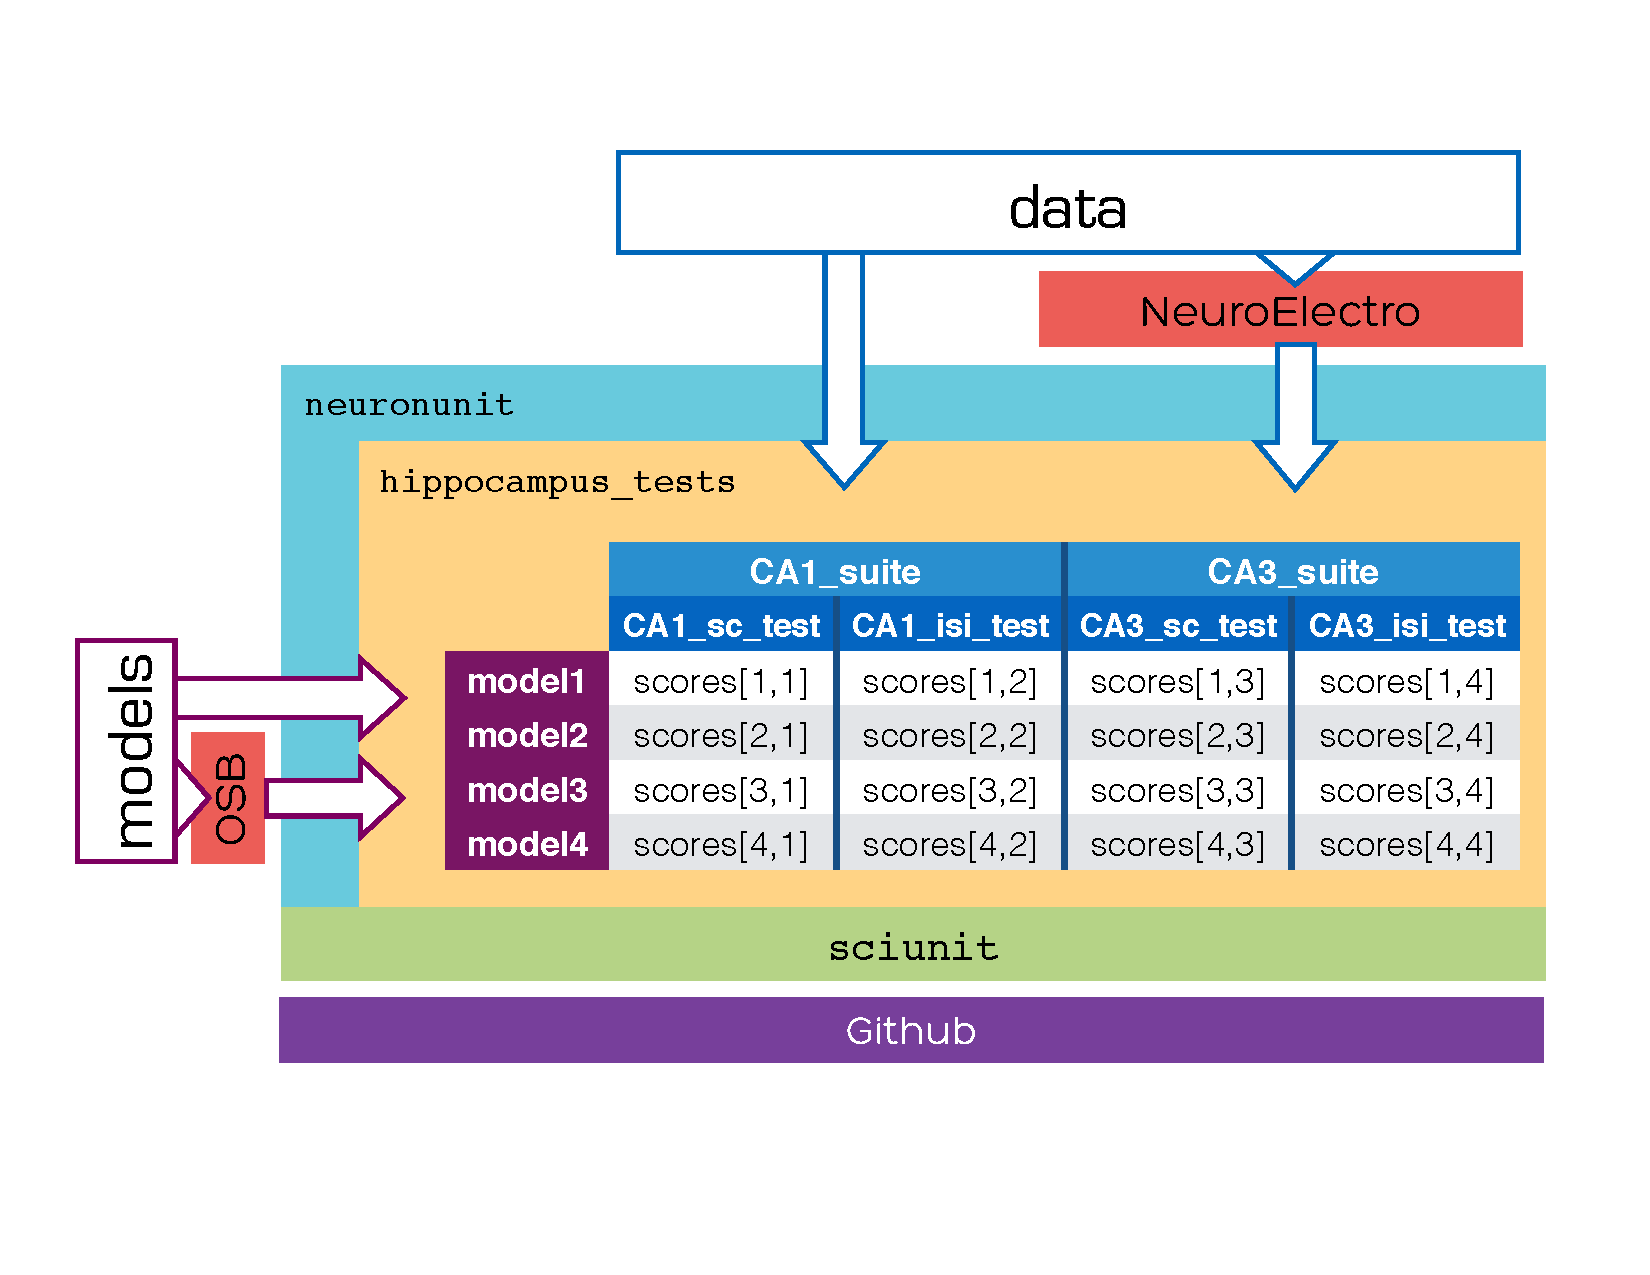
\includegraphics[scale=0.6]{diagram1.pdf}
\vspace{-55px}
\caption{Paper overview.}
\label{fig:sciunit_overview}
\end{figure}
\leavevmode
\vspace{-0px}

Each of these examples has leveraged \emph{ad hoc} infrastructure to support test generation. While the specific criteria used to evaluate models varies widely between disciplines in neuroscience, the underlying test-driven methodology has many common features that could be implemented once. Recognizing this, we have developed a discipline-agnostic framework for developing scientific validation test suites called \textit{SciUnit}\cite{sciunit_url}. To demonstrate the power of this framework and show how it can be used to bridge several existing neuroinformatics tools, we then  developed \textit{NeuronUnit\-}. This library allows scientists to build \textit{SciUnit} tests that validate \text{NeuroML}  models against electrophysiological data collected by the \textit{NeuroElectro Project} \cite{neuroelectro_url}, leveraging facilities from the \textit{NeuroTools} project to..\todo{what does NeuroTools do?}\todo{refer to and describe figure 1}\todo{add caption to figure 1}.% In addition to this open testing toolkit we also provide a library of tests for models of spiking single neurons.  

% Section 2.
\section{Validation Testing with \textit{SciUnit}}
\subsection{Example: Quantitative Single Neuron Modeling Competition}
\begin{figure}
\small
\begin{python}
class SpikeCountTest(sciunit.Test):
  """Tests spike counts produced in response to several current stimuli against observed means and standard deviations. 

  goodness of fit metric: Computes p-values based on a chi-squared test statistic, and pools them using Fisher's method.
  parameters:
    inputs: list of numpy arrays containing input currents (nA)
    means, stds: lists of observed means and standard deviations, one per input
  """
  def __init__(self, inputs, means, stds):
    self.inputs, self.means, self.stds = inputs, means, stds
	
  required_capabilities = [SpikeCountFromCurrent]
	
  def run_test(self, model):
    inputs, means, stds = self.inputs, self.means, self.stds
    n = len(inputs)
    counts = numpy.empty((n,))
    for i in xrange(n):
      counts[i] = model.spike_count_from_current(inputs[i])
    chisquared = sum((counts-means)**2 / means) # An array of chi-squared values.  
    p = scipy.stats.chi2.cdf(chisquared,n-1) # An array of p-values.  
    pooled_p = sciunit.utils.fisherp(p_array) # A pooled p-value.  
    return sciunit.PValue(pooled_p, related_data={
      "inputs": inputs, "counts": counts, "obs_means": means, "obs_stds": stds
    })
\end{python}
\vspace{-5px}
\caption{A single neuron spike count test family implemented using \textit{SciUnit}. This family contains logic common to many different systems, so it is distributed in the \textit{NeuronUnit} repository (see Sec. \ref{sec:neuronunit}).}
\label{fig:rate_test}
\vspace{-15px}
\end{figure}

%Simple executable \emph{validation tests} that compute agreement between a model prediction and an experimental observation.  
We begin by constructing an example validation test suite. 
Suppose we have collected data from an experiment where current stimuli (measured in pA) are delivered to neurons in some brain region, while the somatic membrane potential of each stimulated cell (in mV) is recorded and stored.  
A model claiming to capture this cell type's membrane potential dynamics must be able to accurately predict a variety of features observed in these data.

One simple validation test would ask candidate models to predict the number of action potentials (a.k.a. spikes) generated in response to a stimulus (e.g. white noise), and compare these \emph{spike count} predictions to the distribution observed in repeated experimental trials using the same stimulus. 
In our example, we will determine goodness-of-fit by first calculating a p-value from a chi-squared statistic for each prediction and then combining these p-values using Fisher's method\cite{fisher_statistical_1925}. 

Alongside this \emph{spike count test}, a number of other tests capturing different features of the data can be specified to produce a more comprehensive suite. 
For data of this sort, the QSNMC defined 17 other validation criteria in addition to one based on the overall spike count, capturing features like spike latencies (SL), mean subthreshold voltage (SV), interspike intervals (ISI) and interspike minima (ISM) that can be extracted from the data\cite{jolivet_quantitative_2008}. 
They then defined a combined metric favoring models that broadly succeeded at meeting these criteria, to produce an overall ranking. 
Such combined criteria are simply validation tests that invoke other tests to produce a result.
 
%In many cases, models require no modifications to take the new tests because the same type of model output is being requested.
\subsection{Implementing a Validation Test in \textit{SciUnit}}
Fig. \ref{fig:rate_test} shows how a scientist would implement spike count tests such as the one described above using \textit{SciUnit}. 
A \textit{SciUnit} validation test is an {instance} (i.e. an object) of a Python class implementing the \verbx{sciunit.Test} interface (cf. line 1). 
Here, we show a class \verbx{SpikeCountTest} taking three \emph{parameters} in its constructor (constructors are named \verbx{__init__} in Python, lines 9-10). The meaning of each parameter along with a description of the goodness-of-fit metric used by the test is documented on lines 4-7. 
%For convenience, we also make use of functions provided by the popular NumPy\cite{numpy_url} and SciPy\cite{scipy_url} libraries, although these are not required by \textit{SciUnit}.  
To create a \emph{particular} spike count test, we instantiate this class with particular experimental observations. 
For example, given observations from hippocampal CA1 cells (not shown), we can instantiate a test as follows:
\begin{python}
  CA1_sc_test = SpikeCountTest(CA1_inputs, CA1_means, CA1_stds)
\end{python}
We emphasize the crucial distinction between the \textit{class} \verbx{SpikeCountTest}, which defines a \emph{parameterized family} of validation tests, and the particular \textit{instance} \verbx{CA1_sc_test}, which is an individual validation test because the necessary parameters, derived from data, have been provided. 
As we will describe below, we expect communities to build repositories of such families capturing the criteria used in their subfields of neuroscience so that test generation for a particular system of interest will often require simply instantiating a previously-developed family with particular experimental parameters and data. 
For single-neuron test families like \verbx{SpikeCountTest}, we have developed such a library, called \textit{NeuronUnit} \cite{neurounit_url} (Sec. \ref{sec:neuronunit}). 

Classes that implement the \verbx{sciunit.Test} interface must contain a \verbx{run_test} method that receives a candidate \emph{model} as input and produces a \textit{score} as output. 
To specify the interface between the test and the model (that is, to specify an appropriate scope), the test author provides a list of \emph{capabilities} in the \verbx{required_capabilities} attribute, seen on line 12 of Fig. \ref{fig:rate_test}. 
Capabilities are simply collections of methods that a test may need to invoke to receive relevant data, and are analogous to \emph{interfaces} in e.g. Java \cite{java_interfaces_url}. 
In Python, they are written as classes with unimplemented members. 
The capability required by the test in Fig. \ref{fig:rate_test} is shown in Fig. \ref{fig:capability}. 
In \textit{SciUnit}, classes defining capabilities are tagged as such by inheriting from \verbx{sciunit.Capability}. The test in Figure \ref{fig:rate_test} uses this capability on line 19 to produce a spike count prediction for each input current. 

The remainder of the \verbx{run_test} method implements the goodness-of-fit metric described above, returning an instance of \verbx{sciunit.PValue}, a subclass of \verbx{sciunit.Score} included with \textit{SciUnit}. In addition to the score itself, the returned score object also contains metadata, via the \verbx{related_data} parameter, for  those who may wish to examine the result in more detail. 
In this case we save the input currents, the model outputs and the observed means and standard deviations alongside the score (line 24). 
%We discuss visualization of results in Secs. \ref{sec:scidash_activities} and \ref{sec:scidash_visualization}.

\begin{figure}
\begin{python}
class SpikeCountFromCurrent(sciunit.Capability):
  def spike_count_from_current(self, input): 
    """Takes a numpy array containing current stimulus (in nA) and
    produces an integer spike count. Can be called multiple times."""
    raise NotImplementedError("Model does not implement capability.")
\end{python}
\caption{An example capability specifying a single required method (used by the test in Figure \ref{fig:rate_test}).}
\label{fig:capability}
\vspace{-10px}
\end{figure}

\begin{figure}
\begin{python}
class TrainSpikeCountFromCurrent(sciunit.Capability):
  def train_with_currents(self, currents, counts):
    """Takes a list of numpy arrays containing current stimulus (in nA) and
    observed spike counts. Model parameters should be adjusted based on this
    training data."""
    raise NotImplementedError("Model does not implement capability.")
\end{python}
\caption{Another capability specifying a training protocol (not used by the test in Figure \ref{fig:rate_test}).}
\label{fig:training}
\vspace{-15px}
\end{figure}

\subsection{Models}
Capabilities are \emph{implemented} by models. In \textit{SciUnit}, models are instances of Python classes that inherit from \verbx{sciunit.Model}. Like tests, the class itself represents a family of models, parameterized by the arguments needed in the constructor. A particular model is an object created by supplying the parameters.

A simple {family} of models, \verb{LinearModel}, implementing the capability in Fig. \ref{fig:capability} as well as another capability shown in Fig. \ref{fig:training}, is shown in Fig. \ref{fig:simple_model}. 
Models in this family, \verbx{LinearModel}, produce a spike count by applying a linear transformation to the mean of the provided input current. 
The family is parameterized by a scale factor and offset, both scalars. 
To create a \emph{particular} model, the modeler may choose particular parameter values, just as with test families:
\begin{python}
CA1_linear_model_heuristic = LinearModel(3.0, 1.0)
\end{python}
Here, the parameters to the model were picked by the modeler heuristically, or based on externally-available knowledge. 
An alternative test design to the one in Fig. \ref{fig:rate_test} would add a second required capability (Fig. \ref{fig:training}) and a corresponding training phase to the \verb|run_test| method. 
This design would be relevant only for those models for which parameters can be adjusted without human involvement. 
Whether to build a training phase into the test protocol is a choice left to each modeler. 
Although Fig. \ref{fig:rate_test} does not include a training phase, if training data is available then models that nevertheless implement a training capability (like \verb|LinearModel|) can simply be trained explicitly by calling the capability method just like any other Python method:
\begin{python}
CA1_linear_model_fit = LinearModel()
CA1_linear_model_fit.train_with_currents(CA1_training_in, CA1_training_out)
\end{python}
\begin{figure}
\begin{python}
class LinearModel(sciunit.Model, SpikeCountFromCurrent, 
    TrainSpikeCountFromCurrent):
  def __init__(self, scale=None, offset=None): 
    self.scale, self.offset = scale, offset
    
  def spike_count_from_current(self, input):
    return int(self.scale*numpy.mean(input) + self.offset)

  def train_with_currents(self, currents, counts):
    means = [numpy.mean(c) for c in currents]
    [self.offset, self.scale] = numpy.polyfit(means, counts, deg=1)    
\end{python}
\caption{A simple model that returns a spike count by scaling the mean of the input by a fixed parameter.}
\label{fig:simple_model}
\vspace{-15px}
\end{figure}

Finally, a test is executed against a model instance, using the \verbx{sciunit.judge} function:
\begin{python}
score = sciunit.judge(CA1_sc_test, CA1_linear_model_heuristic)
\end{python}

Collection of tests with mutually coherent requirments, i.e. various summaries of the available empirical data, can form test suites.
The following is a test suite that could be used for a simplified version of the QSNMC:  
\begin{python}
CA1_suite = sciunit.TestSuite([CA1_sc_test, CA1_sl_test, CA1_sv_test, CA1_isi_test, CA1_ism_test])
\end{python}
When a test suite is executed against a model, it produces summary data that can be shown on the console or visualized by other tools, such as the web application described in Sec. \ref{sec:scidash}.

% Section 3.
\section{Results}

\subsection{\textit{NeuronUnit}: A Suite of Tests for Neurophysiology}\label{sec:neuronunit}
By using machine-readable models from Open Source Brain (OSB), and machine-readable data from resources like The NeuroElectro Project\cite{neuroelectro_url}, we have produced a suite of data-driven validation tests in \textit{NeuronUnit}, as well as tools for capability implementation, and model interfaces for a representative set of canonical neurophysiology models, all publicly available. 

\label{sec:neuronunit_acitivities}
Here we describe standard neuroinformatics tools we have adopted to develop \textit{NeuronUnit}\cite{neurounit_url}.  

\subsubsection{Models from NeuroML}\label{sec:neuroml_models}
NeuroML is a standardized model description language for neuroscience \cite{gleeson_neuroml:_2010}. 
It permits many neurophysiological/neuroanatomical models to be described in a simulator-independent fashion, and executed across many popular simulators due to inter-conversion capabilities of the NeuroML API. 
Because NeuroML is an XML specification, model descriptions can be validated for correctness and queried for model properties and components, exposing potential capabilities. 
It is ideal for model sharing, curation, and for answering both \textit{what} and \textit{how} programatically.  

NeuroConstruct\cite{neuroconstruct_url,gleeson_neuroconstruct:_2007} is a simulation manager that takes NeuroML models and hands off simulation to supported simulators. 
\textit{NeuronUnit} offers a \verbx{sciunit.Model} subclass called \verbx{NeuroConstructModel}, instantiated with the path to a NeuroML model.  
Because NeuroML can describe such a wide range of models, \verbx{NeuroConstructModel} makes few assumptions about them: that each one is \verbx{TimeIntegrable}, and \verbx{HasMembranePotential}.  
It is subclassed to test \textit{specific} NeuroML models (Fig. \ref{fig:ca1_model}). 

The Open Source Brain project (OSB,\cite{osb_url}) curates many models described in NeuroML. 
OSB-curated projects are converted from their native format into NeuroML, and run on major neural simulators\cite{neuron_url,genesis_url,nest_url,moose_url}. 
Concordance between model output (beginning with the NeuroML description) and reference output (from native simulator source files) is reported for each model. 
Thus, OSB is an excellent source of models that, in addition to being open source, are sufficiently described to enable validation. 
The hippocampal CA1 pyramidal cell is commonly modeled, and we implement one such model hosted on OSB\cite{osb_ca1_url} by simply declaring a \verbx{CA1PyramidalCellModel} class, inheriting from \verbx{NeuroConstructModel}.  
This basic implementation simply ``wraps'' the components of the existing model, with simulator interaction taken care of by \verbx{NeuroConstructModel} methods; 
thus, only the code shown in Fig. \ref{fig:ca1_model} is required. 
All OSB models, and indeed any NeuroML model, can be tested similarly. 
Working together with OSB is part of our \textbf{first collaboration}, and our integration efforts can be publicly tracked\cite{neuroconstruct_rgerkin_url}.  

Spanning a range of scales and original development environments, all OSB models are formally described using NeuroML, as are all model components and sub-components, such as cells, ion channels, calcium stores, etc. 
These models are regularly executed on OSB servers to ensure that their output remains consistent as they are updated. 
Therefore, OSB can confirm that they \textit{do} work, while linked journal articles, on-site wiki, and code inspection can establish \textit{how} they work. 
However, there is no mechanism for establishing \textit{how well} they work, i.e. how well the models accord with data. 
\textit{NeuroUnit} fills this gap by helping OSB (and the larger biology community) assess models using data-driven tests. 
\textit{SciUnit} can be applied similarly to other neuroscience (or biology) sub-disciplines using \textit{NeuronUnit} analogues written by the corresponding communities.    

\begin{figure}
\begin{python}
class CA1PyramidalCellModel(NeuroConstructModel):
	"""CA1 Pyramidal Cell model from Open Source Brain."""
	def __init__(self,**kwargs):
		project_path = neuroconstruct.get_path("hippocampus","CA1_pyramidal_neuron","CA1PyramidalCell","neuroConstruct")
		models.NeuroConstructModel.__init__(self,project_path,**kwargs)
\end{python}
\vspace{-5px}
\caption{A model class corresponding to a CA1 Pyramidal Cell model from Open Source Brain}
\label{fig:ca1_model}
\vspace{-15px}
\end{figure}

\subsubsection{Capabilities from NeuroTools}
NeuroTools\cite{neuralensemble_url} is a Python library supporting tasks associated with analysis of neural data (or model output), such as membrane potential time series, spike trains, etc. 
It is an open source and actively developed project, containing reliable algorithms on which to base neurophysiology tests.

We use NeuroTools to implement \textit{SciUnit} capabilities in \textit{NeuronUnit}. 
For example, an \verbx{AnalogSignal} object (e.g. a membrane potential time series) from NeuroTools has a threshold detection method that returns a NeuroTools \verbx{SpikeTrain} object. 
A \textit{NeuronUnit} \verbx{HasSpikeTrain} Capability requires that the method \verbx{getSpikeTrain} be implemented. 
\verbx{NeuroConstructModel} does so by placing the object method \verbx{AnalogSignal.threshold_detection} inside \verbx{getSpikeTrain}. 
Many such NeuroTools objects are similarly exchanged between \verbx{NeuroConstructModel} methods. 
This simplifies test writing, since basic model output properties are obtained trivially using NeuroTools object methods, and these NeuroTools objects are easily extracted from model output using candidate models subclassing \verbx{NeuroConstructModel}.  

\subsubsection{Reference Data for Tests from NeuroElectro}
Answering \textit{how well} requires validation testing against data. 
The NeuroElectro project\cite{neuroelectro_url} is an effort to curate all published single cell neurophysiology data\cite{tripathy_neuroelectro:_2012}.  
Currently, up to 27 electrophysiological properties are reported for 93 cell types, spanning $>$ 2000 single pieces of published data extracted from article tables. 
We have made it easy to construct \textit{NeuronUnit} tests using the NeuroElectro API to get reference data. 
Tests can be based upon data from single journal articles, or from ensembles of articles with a common theme (e.g. about a particular neuron type). 
The former is illustrated in Figure \ref{fig:neuronunit_example}. 
Associated statistics of that data (e.g mean, standard error, and sample size) are attached and enable judgement of model output according to a chosen scoring mechanism. 
While NeuroElectro alone cannot judge all model aspects, it can serve to validate basic features of many neurophysiology models, such as resting membrane potential, action potential width, after-hyperpolarization amplitude, etc. 
As NeuroElectro is the only publicly curated source of such data, it represents a key component for \textit{NeuronUnit} test constuction.  
Continued development of the NeuroElectro API, through which data are systematically exposed to test authors, represents our \textbf{second collaboration}\cite{neuroelectro_dev_url}.  

\subsection{\textit{SciDash}: A community web application}\label{sec:scidash}
A collection of tests, models, and test records can summarize the current state of modeling in a research area.  
Community-oriented cyberinfrastructure to support the creation and summarization of such collections is essential.
We used a service called \textit{SciDash} \cite{scidash_url} for coordinated development of software repositories.

\begin{wrapfigure}[18]{r}{0.45\textwidth}
\center
\vspace{-10px}
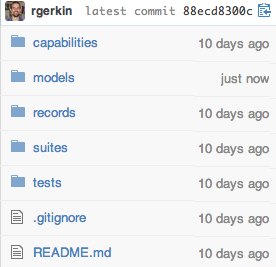
\includegraphics[scale=0.72]{scidash_github.png}
\caption{A \textit{SciDash} repository on GitHub}
\label{fig:scidash_repo}
\end{wrapfigure}
\vspace{-10px}
\leavevmode

\textit{SciDash} exists in three layers.
The \textbf{first layer} is completely under the control of individual developer communities, and consists of git repositories \cite{ram_git_2013} stored on GitHub \cite{github_url}. 
\textit{SciDash} identifies all similarly structured repositories (by tracking the lineage of a vanilla \textit{SciDash} repository above using the GitHub API).
This list of repositories is indexed by \textit{SciDash} to form the \textbf{second layer}, an overview of the state of all \textit{SciDash} repositories on GitHub.  
This index is searchable and filterable on the \textit{SciDash} website to identify repositories of interest to a particular research community.  
The \textbf{third layer} is a ``dashboard'' view of the state of a field, visible through a matrix of records for model/test combinations in a GitHub repository (Fig. \ref{fig:scidash_repo}). 
Test records are visualized as a ``record matrix'' composed of large numbers of model/test combinations (Fig. \ref{fig:scidash_matrix}).  
Each row in this matrix contains results for all tests taken by one model and serve as clear evidence of that model's scope and validity.  
Hyperlinks in the record matrix point to models, tests, and records available on GitHub. 
Each record links to test records (stored in the repository), displaying line-by-line the executed code and intermediate output statements, as well as the underlying models and tests.   

\begin{figure}%[18]{r}{1\textwidth}
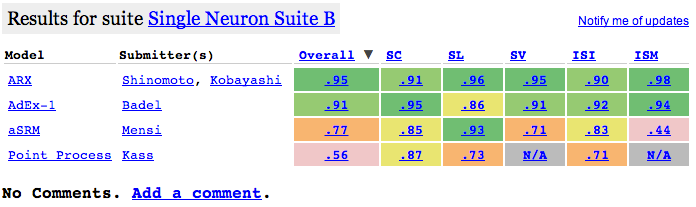
\includegraphics[scale=0.65]{table.png}
\caption{A \textit{SciDash} record matrix}
\label{fig:scidash_matrix}
\vspace{-15px}
\end{figure}
\vspace{-10px}
\leavevmode

% Section 4.
\section{Discussion}
The validation criteria is made explicit in the specification of a test, so modelers need not guess which criteria are being used to validate or invalidate their model. 
Validation criteria are subject to debate (indeed, the QSNMC criteria changed between 2007 and 2008 due to such debates), and neuroscientists who wish to promote different criteria need only derive alternative tests. A community consensus will slowly emerge in the form a commonly-accepted test suite (see Sec. \ref{sec:scidash}). \todo{integrate this somewhere down here}

\subsection{A Complete Pipeline}
Although the tools described in Sec. \ref{sec:neuronunit_acitivities} do not exhaust the possible sources of models, capabilities, and test data, they provide an immediate point of entry into the neurophysiology community and a powerful demonstration of our proposal. 
In the \textit{NeuronUnit} repository\cite{neurounit_url} is a runnable script (\textit{examples.py}) demonstrating a complete testing pipeline. 
It (1) selects an OSB model; 
(2) simulates it using NeuroConstruct; 
(3) tests the widths of the resulting action potentials, extracted and computed using NeuroTools, against NeuroElectro data downloaded on-the-fly, using a \textit{NeuronUnit} test class called \verbx{SpikeWidthTestDynamic}; 
and (4) computes and prints a test score (Figure~\ref{fig:neuronunit_example}).

\begin{figure}
\begin{python}
# Interface with neuroelectro.org to search for spike widths of CA1 Pyramidal cells. 
reference_data = NeuroElectroSummary(neuron={'id':85}, ephysprop={'id':23})
reference_data.get_values()  # Get summary data for the above. 
model = CA1PyramidalCellModel(population_name="CG_CML_0") # Initialize the model with some parameters.
test = SpikeWidthTestDynamic( # Initialize the test.    
	reference_data = {'mean':reference_data.mean, 'std':reference_data.std}, # Summary statistics from the reference data
	model_args = {'current':40.0}, # Somatic current injection in pA.  
	comparator = ZComparator), # A comparison class that implements a Z-score.  
result = sciunit.judge(test,model) # (1) Check capabilities, (2) take the test, (3) generate a score and validate it, (4) bind the score to model/test combination. 
result.summarize() # Summarize the result.  
\end{python}
\caption{Working example of a testing in \textit{NeuronUnit}}
\label{fig:neuronunit_example}
\vspace{-15px}
\end{figure}

\subsection{Creating New Models, Capabilities, and Tests}
\textit{NeuronUnit} provides base classes to enable rapid generation of models, capabilities, and tests for neurophysiology data. 
However these objects can also be created from scratch, requiring only adherence to the \textit{SciUnit} interface. 
For example, a Model could implement an \verbx{integrate} capability method by wrapping execution of a MATLAB script and a \verbx{get_spikes} capability method by parsing a .csv file on disk; 
a Test could be initialized using empirical spike rates collected in the lab.  
While this does not meet our idealized vision of development and testing, in practice this may be a common scenario. 
As part of our outreach efforts (Sec. \ref{sec:broader_impacts}) we will train modelers in the use of this framework, and encourage them to use it as part of their workflow of choice. 
Adoption of \textit{SciUnit} into traditional, custom workflows would be reflected in the Methods sections of articles.  

\subsubsection{Collaboration}
Community-moderated comments on GitHub will allow test-makers and test-takers to discuss issues associated with test suites. 
On GitHub, these takes the form of ``issues,'' commit messages, and comments surrounding merge requests from forked repositories. 
Thus, disagreements about the appropriateness of a test can be openly aired and in many cases resolved. 
The \textit{SciDash} website itself can also support public comment to extend the features of GitHub. 
More importantly, we will enable sorting and filtering of \textit{SciDash} results by repository statistics, e.g. the volume of activity and the number of followers, via the GitHub API. 
This will allow the most important test suites, as judged by each community, to be featured prominently on \textit{SciDash}. 
Simple tagging should enable filtering by subject matter. 
We also will support open authentication via existing web applications (Google, Twitter, etc.), lowering the barrier to participation.  

\subsection{Participation from Modeling Communities}
Modelers may not want to expose model capabilities, a requirement of test-taking.  
We anticipate four solutions: \textbf{First}, interfacing a model to \textit{SciUnit} requires only implementing selected model capabilities. 
Often this means identifying native model procedures that satisfy a capability, and wrapping their functionality. 
This can require as little as one line of code. 
Importantly, the modeler is not required to expose or rewrite any model flow control. 
\textbf{Second}, we support multiple environments automatically by using NeuroML\cite{gleeson_neuroml:_2010}, and other simulator-independent model descriptions are possible for other domains. 
Automated generation of NeuroML from native model source code is in development (Gleeson, personal communication); for the popular NEURON simulator\cite{neuron_url}, this functionality is already mature and in use. 
This minimizes modeler effort for a large and growing number of models. 
\textbf{Third}, modelers have an incentive to demonstrate publicly their models' validity. 
Participation in public modeling competitions (Sec. \ref{sec:existing_efforts}) demonstrates this incentive. 
\textbf{Fourth}, modelers have an incentive to use \textit{SciUnit} during development (see TDD, above) to ensure that ongoing development preserves correspondence between model and data. 
A popular test suite can represent a ``gold standard'' by which progress during development is judged.

\subsection{Participation from Experimental Communities}
Experimentalists may not want to write tests derived from their data.  We anticipate four solutions: \textbf{First}, tests require no special data formatting; only a list of required  capabilities (for selecting eligible models), optional metadata (as run-time arguments), and a statistical data summary (for scoring tests) are required.  A unit test is focused and does not require arbitrary computations on data.  For example, suppose intracellular current injection evokes 100 action potentials, the width of which is of interest.  Writing the test consists of selecting \verbx{ReceivesCurrent} and \verbx{ProducesActionPotentialShape} capabilities (one line of code each), computing the mean and variance of action potential widths (one line of code), specifying current injection parameters, e.g. amplitude and duration (two lines of code), and selecting a scoring mechanism from \verbx{sciunit.scores}, e.g. (colloquially) ``Must be $<$ 1 standard deviation of the mean'' (one line of code).  This example can be found in \verbx{NeuronUnit.tests.SpikeWidthTest}; heavy-lifting is done by the interface.
\textbf{Second}, data-sharing is becoming accepted, and test-writing can be distributed across scientists, including non-experimentalists with other aims such as analysis or modeling. 
\textbf{Third}, many tests can be automatically generated using the NeuroElectro API, and the continued emergence of such data-aggregation initiatives will expand these possibilities. 
\textbf{Fourth}, an incentive to write tests for one's data exists: the ability to identify models that give the data clear context and impact. 

\subsection{Diversity of Levels and Kinds of Models and Data}
The diversity of topics in biology is vast. 
\textbf{First}, we address this by providing an interface allowing modelers to express specific capabilities.  
This capability set determines the range of eligible tests.  Scale hierarchies are embedded in capability inheritance.  =
For example, \verbx{HasActionPotentials} inherits from \verbx{HasNeurons}, and \verbx{HodgkinHuxley} inherits from \verbx{VoltageGated}. 
Thus, incompatibility of a test-requiring-action-potentials for a model-lacking-neurons is known without explicit tagging. 
\textbf{Second}, NeuroML naturally addresses diversity of scales because it is organized hierarchically, in ``levels.''  
Models can be sub- or supersets of other models; similarly for SBML\cite{sbml_url,hucka_systems_2003}, a general systems biology markup language. 
\textbf{Third}, cross-level testing can use ``Representional Similarity Analysis'' (RSA)\cite{kriegeskorte_representational_2008}, requiring only that a model respond to defined inputs (e.g. stimuli). 
A ``similarity matrix'' for input responses defines a unique model signature, and can serve as intermediate test output. 
Goodness-of-fit between similarity matrices for model and experiment determines test scores; 
these matrices are independent of model scale because their size depends only on test inputs, not system detail.  

\subsection{Arbitrary Scoring Criteria for Tests}
A test first assesses goodness-of-fit, and applies a normalization (e.g. pass/fail, 0.0-1.0) to generate a score. 
Arbitrary choices at both stages may benefit some models over others.  \textbf{First}, however, rank-ordering is constant across many goodness-of-fit metrics, meaning that choice of metric will rarely cause an otherwise passing model to fail and vice versa. 
For example, given a data mean and variance, ordering model output by Z-score or p-value will yield the same relative ranking of models. 
Indeed, rank ordering of models may prove more valuable than test scores themselves. 
\textbf{Second}, suite repositories are open (e.g. Fig. \ref{fig:scidash_repo}), so tests can be cloned and new statistical choices implemented. 
Statistics as applied to neuroscience have been notoriously ``fast and loose''; 
identification and correction of flawed methodology is becoming increasingly common\cite{button_power_2013,kriegeskorte_circular_2009,galbraith_study_2010,fish_fmri_url}, and is accelerated by an open framework. 
The community can judge which test version is most appropriate, i.e. what a model \textit{should} do -- this process documented via standard moderation techiniques used on GitHub -- and the \textit{SciUnit} framework determines whether the model \textit{does} it.  

\subsection{Reliability of Data Underlying Tests}
Unreliable data can undermine model validation. 
\textbf{First}, the community must evaluate experimental design and methods, discounting data produced using questionable techniques. 
GitHub supports community moderation, permitting users to comment on tests, indicating their concerns. 
Suite repository popularity, by which \textit{SciDash} results can be filtered, can reflect consensus. 
Experimental metadata also constrains a test's relevance, so test writers should select data with metadata appropriate to the system being modeled, and attach the metadata to resulting test scores. 
Metadata can also be expressed as Capabilities, e.g. \verbx{At37Degrees} or \verbx{Calcium3mM}; and tests can require that models express them. 
Such capabilities require no implementation, so the model definition must only inherit them. 
\textbf{Second}, models cannot perfectly reproduce data that is itself a random draw from a ``true'' distribution. 
Uncertainty in data must be made explicit, by asking how well a data set validates its own experimental replications\cite{kriegeskorte_representational_2008}. 
The degree of such ``self-validation'' represents the upper limit of what a model can be expected to achieve, and should represent a ``perfect'' score.  

\subsection{Occam's Razor}
All things being equal, simpler models are better. 
Model complexity has many definitions, so \textit{SciDash} will report several complexity metrics\cite{mccabe_complexity_1976}, including: 
1) model length; 2) memory use; 3) CPU load; 4) \# of capabilities. 
\textit{SciDash} will report the model validity vs complexity tradeoff in tabular form (e.g. Table \ref{table:record_matrix}), and in a scatter plot, with the ``best'' models being in the high validity / low complexity corner of the plot. 
The set of models which \textit{dominate} all others, i.e. that have the highest validity for a given complexity, can be represented as a ``frontier'' in such a scatter plot, a visualization familiar from the symbolic regression package Eureqa\cite{schmidt_distilling_2009}.  

\subsection{Expansion Into Other Areas of Biology}
After covering neurophysiology, we would like \textit{SciUnit} to be applied across neuroscience and in other biological sciences. 
The framework is discipline-agnostic, so community participation and model description are the only obstacles. 
Community participation begins with enumerating the capabilities relevant to a sub-discipline, and then writing tests. 
Model description can expand within NeuroML (which already covers multiple levels within neuroscience) and tools for capability implementation can incorporate libraries for neuroimaging (NiBabel\cite{nibabel_url}), neuroanatomy (NeuroHDF,\cite{neurohdf_url}) and other sub-disciplines. 
SBML\cite{hucka_systems_2003,sbml_url} will enable expansion beyond neuroscience, facilitated by parallel efforts among NeuroML developers to interface with it (Crook, unpublished). 
One intriguing possiblity is applying \textit{SciUnit} to the OpenWorm project\cite{open_worm_url}, which through open, collaborative development seeks to model the entire organism C. elegans.  

\section{Acknowledgements}
We thank Sharon Crook, Jonathan Aldrich, Shreejoy Tripathy, and Padraig Gleeson for their support of this project.  
The work was supported in part by grant R01MH081905 from the National Institute of Mental Health. 
The content is solely the responsibility of the authors and does not necessarily represent the official views of the National Institutes of Health.

\bibliographystyle{unsrt}
\bibliography{references,references_crook,urls,references_ja}
%\listoftodos
\end{document}

